\chapter{Счётчик команд}

Счётчик команд --- это регистр, который хранит номер выполняемой процессором команды.
Сами команды хранятся в памяти. Процессор выполнив одну, переходит к следующей.
Следовательно, счётчик команд нужно каждый раз увеличивать на единицу.

\section{Практикум}


\section{Циклический инкремент регистра}

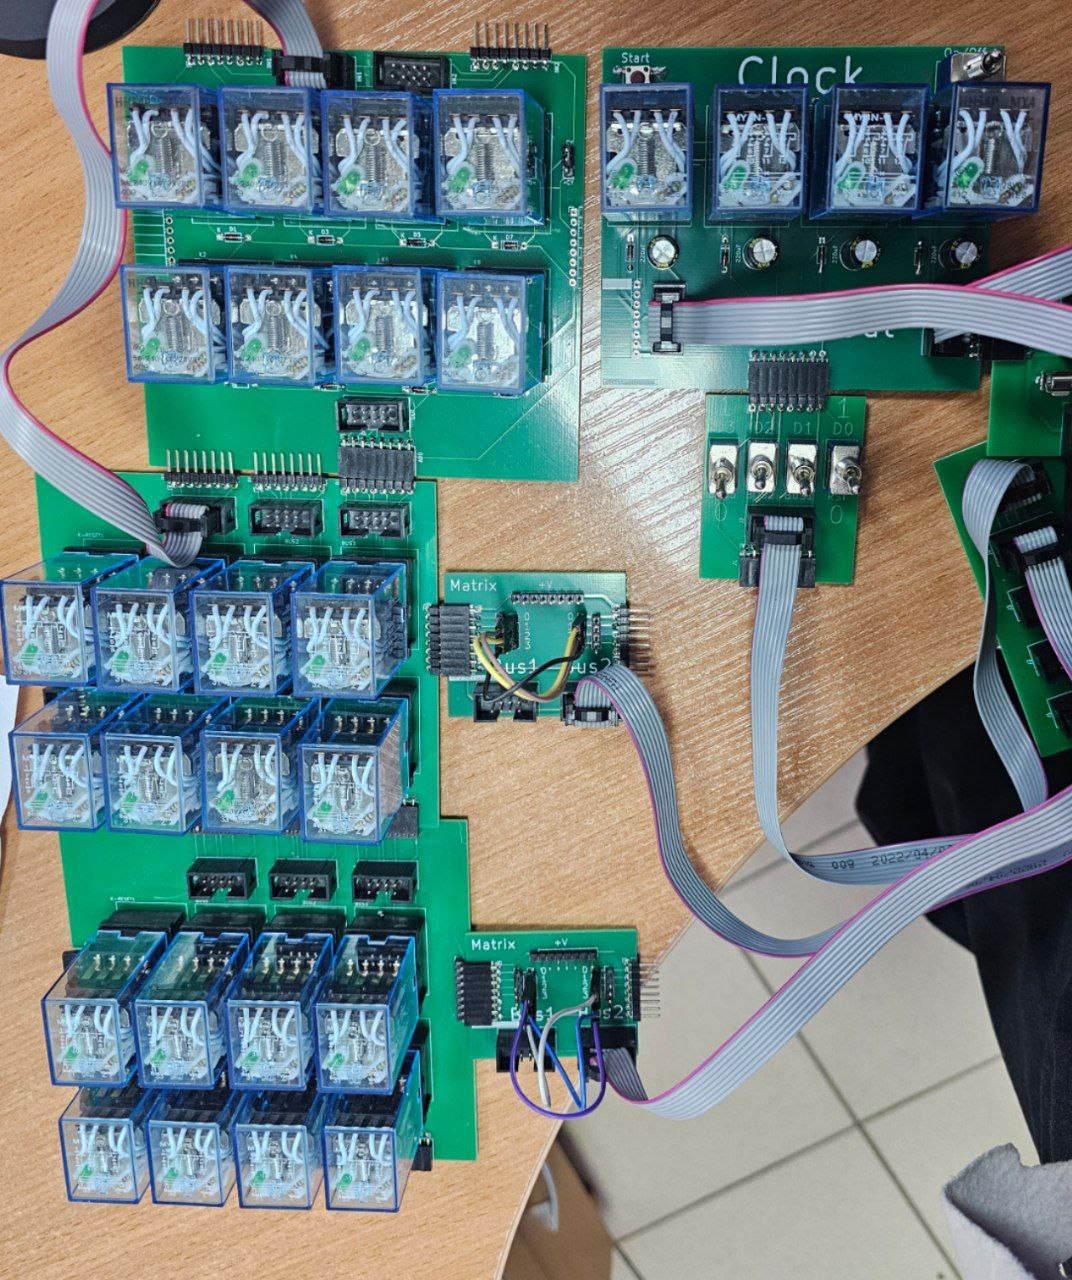
\includegraphics[width=0.5\columnwidth]{photo/increment_loop.jpg}


Список модулей:
\begin{itemize}
    \item Модуль переключателей: \modulesswitches{1} штука
    \item Сумматор: \modulesadder{1} штука
    \item Регистровый модуль: \modulesregister{2} штуки
    \item Тактовый генератор: \modulesclock{1} штука
    \item Кросс-модуль: \modulesmatrix{2} штуки
\end{itemize}

\section{Циклический инкремент регистра и выборка команды из ПЗУ}

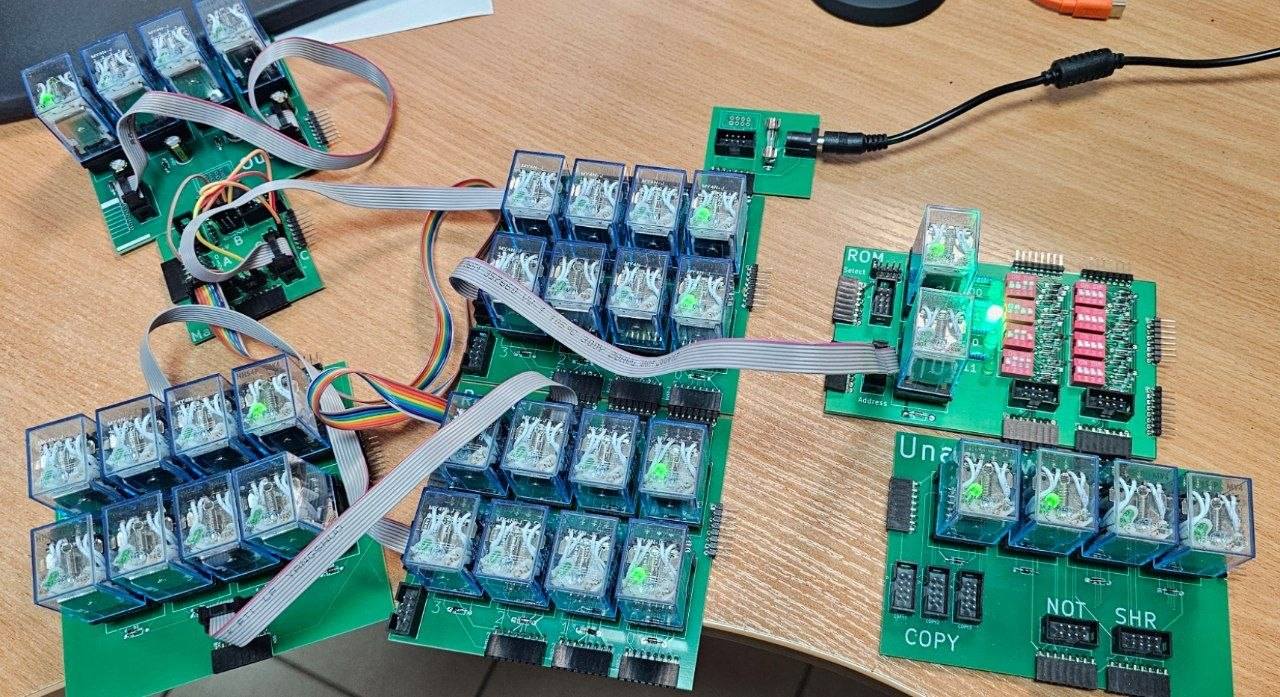
\includegraphics[width=0.5\columnwidth]{photo/rom_pc.jpg}

Список модулей:
\begin{itemize}
    \item ПЗУ: \modulesrom{1} штука
    \item Сумматор: \modulesadder{1} штука
    \item Регистровый модуль: \modulesregister{2} штуки
    \item Тактовый генератор: \modulesclock{1} штука
    \item Кросс-модуль: \modulesmatrix{1} штука
    \item Модуль унарных операций: \modulesunary{1} штука
\end{itemize}

\section{Загрузка команды из ПЗУ в регистр}


\section{Игра <<Лабиринт>>}

Регистр показывает текущее положение в лабиринте. Игрок с помощью тумблеров указывает направление движения.
Затем в регистр-позицию загружается новое значение из ПЗУ по адресу старое положение + направление.
Задача дойти до ячейки {\tt 0xf}.

